%%%%
%% Load the class. Put any options that you want here (see the documentation
%% for the list of options). The following are samples for each type of
%% thesis:
%%
%% Note: you can also specify any of the following options:
%%  logo: put a University of Edinburgh logo onto the title page
%%  frontabs: put the abstract onto the title page
%%  deptreport: produce a title page that fits into a Computer Science
%%      departmental cover [not sure if this actually works]
%%  singlespacing, fullspacing, doublespacing: choose line spacing
%%  oneside, twoside: specify a one-sided or two-sided thesis
%%  10pt, 11pt, 12pt: choose a font size
%%  centrechapter, leftchapter, rightchapter: alignment of chapter headings
%%  sansheadings, normalheadings: headings and captions in sans-serif
%%      (default) or in the same font as the rest of the thesis
%%  [no]listsintoc: put list of figures/tables in table of contents (default:
%%      not)
%%  romanprepages, plainprepages: number the preliminary pages with Roman
%%      numerals (default) or consecutively with the rest of the thesis
%%  parskip: don't indent paragraphs, put a blank line between instead
%%  abbrevs: define a list of useful abbreviations (see documentation)
%%  draft: produce a single-spaced, double-sided thesis with narrow margins
%%
%% For a PhD thesis -- you must also specify a research institute:
\documentclass[phd,aiai,twoside]{infthesis}

%% Put any \usepackage commands you want to use right here; the following is 
%% an example:
\usepackage{natbib}

\title{Probabilistic Inference via Weighted Model Counting: Algorithms, Encodings, and Random Instances}
\author{Paulius Dilkas}

\abstract{%
  This doctoral thesis will present the results of my work into the
  reanimation of lifeless human tissues.
}

\begin{document}

\begin{preliminary}

\maketitle

\begin{acknowledgements}
  Many thanks to my mummy for the numerous packed lunches; and of course to Igor, my faithful lab assistant.
\end{acknowledgements}

\standarddeclaration

%% Finally, a dedication (this is optional -- uncomment the following line if
%% you want one).
% \dedication{To my mummy.}

\tableofcontents

%% If you want a list of figures or tables, uncomment the appropriate line(s)
% \listoffigures
% \listoftables

\end{preliminary}

\chapter{Introduction}

\begin{itemize}
\item What is probabilistic inference?
\end{itemize}

\section{Thesis Structure}

\begin{enumerate}
\item Testing algorithms across a wide range of problem instances is crucial to ensure the validity of any claim about one algorithm's superiority over another. However, when it comes to inference algorithms for probabilistic logic programs, experimental evaluations are limited to only a few programs. Existing methods to generate random logic programs are limited to propositional programs and often impose stringent syntactic restrictions. We present a novel approach to generating random logic programs and random probabilistic logic programs using constraint programming, introducing a new constraint to control the independence structure of the underlying probability distribution. We also provide a combinatorial argument for the correctness of the model, show how the model scales with parameter values, and use the model to compare probabilistic inference algorithms across a range of synthetic problems. Our model allows inference algorithm developers to evaluate and compare the algorithms across a wide range of instances, providing a detailed picture of their (comparative) strengths and weaknesses.
\item Weighted model counting (WMC) has emerged as the unifying inference mechanism across many (probabilistic) domains. Encoding an inference problem as an instance of WMC typically necessitates adding extra literals and clauses. This is partly so because the predominant definition of WMC assigns weights to models based on weights on literals, and this severely restricts what probability distributions can be represented. We develop a measure-theoretic perspective on WMC and propose a way to encode conditional weights on literals analogously to conditional probabilities. This representation can be as succinct as standard WMC with weights on literals but can also expand as needed to represent probability distributions with less structure. To demonstrate the performance benefits of conditional weights over the addition of extra literals, we develop a new WMC encoding for Bayesian networks and adapt a state-of-the-art WMC algorithm \textsf{ADDMC} to the new format. Our experiments show that the new encoding significantly improves the performance of the algorithm on most benchmark instances.
\item Weighted model counting (WMC) is a powerful computational technique for a variety of problems, especially commonly used for probabilistic inference. However, the standard definition of WMC that puts weights on literals often necessitates WMC encodings to include additional variables and clauses just so each weight can be attached to a literal. This paper complements previous work by considering WMC instances in their full generality and using recent state-of-the-art WMC techniques based on pseudo-Boolean function manipulation, competitive with the more traditional WMC algorithms based on knowledge compilation and backtracking search. We present an algorithm that transforms WMC instances into a format based on pseudo-Boolean functions while eliminating around \SI{43}{\percent} of variables on average across various Bayesian network encodings. Moreover, we identify sufficient conditions for such a variable removal to be possible. Our experiments show significant improvement in WMC-based Bayesian network inference, outperforming the current state of the art.
\item TODO
\item TODO
\end{enumerate}
 % 5-14 pages (9 on average)
% 11-45 pages (27 on average)
% aim for 2-5 pages for each major section
\chapter{Background}

TODO: outside of specific sections, have a one-paragraph introduction before and a one-paragraph summary at the end.

\section{Propositional Logic} \label{sec:proplogic}

TODO: explain $\bot$, $\top$, and $\equiv$ (also the term `equivalence').

In this section, we briefly introduce the fundamentals of propositional logic and describe some logic-based computational problems. We refer the reader to the book by \cite{DBLP:books/daglib/0029942} for a more detailed introduction to logic and its role in computer science.

An \emph{atomic proposition} (also known as \emph{atom} and \emph{Boolean/logical/propositional variable}) is a variable with two possible (truth) values: true and false. Unless specified otherwise, we will refer to atoms as \emph{variables}. A \emph{formula} is any well-formed expression that connects variables using the following Boolean/logical operators (and parentheses): negation ($\neg$), disjunction ($\lor$), conjunction ($\land$), (material) implication ($\Rightarrow$), and equivalence (i.e., material biconditional) ($\Leftrightarrow$). A \emph{literal} is either a variable or its negation, respectively called \emph{positive} and \emph{negative} literal. A \emph{clause} is a disjunction of literals.\footnote{In the context of logic programs, the word \emph{clause} is used differently (see \cref{sec:lp,chapter:randomlps}).} A formula is in \emph{conjunctive normal form} (CNF) if it is a conjunction of clauses, and it is in $k$-CNF if every clause has exactly $k$ literals. Many other normal forms and ways to represent propositional formulas are covered in \cref{sec:kc}.

An \emph{interpretation} (also known as a \emph{variable assignment}) of a formula $\phi$ is a map from the variables of $\phi$ to the set $\{\, \text{true}, \text{false} \,\}$. A \emph{model} is an interpretation under which $\phi$ evaluates to true. A formula is \emph{satisfiable} if it has at least one model.

Throughout the thesis, we use set-theoretic notation for many concepts in logic such as clauses and formulas in CNF (e.g., we write $c \in \phi$ to mean that clause $c$ is one of the clauses of formula $\phi$). However, this does not automatically mean that we assume no duplicates---whether or not that is the case is clarified on a case-by-case basis.

\begin{example} \label{example:logic}
  Formula $\phi \coloneqq (\neg a \lor b) \land a$ has two variables $a$ and $b$, is in CNF, and contains two clauses. The first clause $\neg a \lor b$ has a negative literal $\neg a$ and a positive literal $b$. Since $\phi$ has two variables, it also has four interpretations. Interpretation $\{\, a \mapsto \text{true}, b \mapsto \text{true} \,\}$ is a model, so $\phi$ is satisfiable. An equivalent set-theoretic representation of $\phi$ is $\{\, \{\, \neg a, b \,\}, \{\, a \,\} \,\}$.
\end{example}

\subsection{Logic-Based Computational Problems} \label{sec:logicproblems}

We begin with a description of \SAT{} and some of its extensions. Given a propositional formula\footnote{Unless stated otherwise, formulas for \SAT{} and other similar problems are assumed to be in CNF.}, \SAT{} asks whether the formula is satisfiable. \SAT{} (also known as \emph{propositional/Boolean satisfiability}) is the first problem shown to be \NP-complete \citep{DBLP:conf/stoc/Cook71,levin1973universal}. Motivated by many real-life problems that were found to be reducible to \SAT{}, research in \SAT{} solving produced algorithms that can efficiently tackle large instances despite the exponential worst-case time complexity \citep{DBLP:series/faia/2009-185}.

Instead of satisfying all clauses, one can attempt to find an interpretation that satisfies the maximum number of clauses---this problem is called Max\SAT{} \citep{bacchus2021maximum,DBLP:series/faia/LiM09}. It is an \NP-hard optimisation problem that (in its most general form) attaches a (potentially infinite) cost for failing to satisfy each clause and seeks to minise total cost.

\#\SAT{}, or \emph{(propositional) model counting}, asks to count the number of models of a formula \citep{DBLP:series/faia/GomesSS09}. \#\SAT{} is the canonical \#\P-complete problem with many applications in areas such as planning and probabilistic reasoning. $\#\exists\SAT{}$, or \emph{projected model counting}, selects a subset of variables called \emph{priority variables} \citep{DBLP:conf/sat/AzizCMS15}. The task is then to count the number of assignments of values to priority variables that can be extended to models. The extension of \#\SAT{} most relevant to our work is called \emph{weighted model counting} (WMC). Given a propositional formula $\phi$ and a \emph{weight function} $w$ from the literals of $\phi$ to non-negative real numbers, WMC asks to compute
\[
\mathrm{WMC}(\phi) = \sum_{\omega \models \phi} \prod_{\omega \models l} w(l),
\]
where the summation is over all models $\omega$ of $\phi$, and the product is over all literals of $\omega$ \citep{DBLP:journals/ai/ChaviraD08}. Lastly, both \#\SAT{} and WMC have been extended to first-order logic \citep{DBLP:conf/ijcai/BroeckTMDR11}---this is the topic of \cref{chapter:wfomc}.

\begin{example} \label{example:wmc1}
  The model count of the formula in \cref{example:logic} is equal to one. With a weight function $w \coloneqq \{\, a \mapsto 0.7, \neg a \mapsto 0.2, b \mapsto 0.8, \neg b \mapsto 0.7 \,\}$, the WMC of the same formula is $0.7 \times 0.8 = 0.56$.
\end{example}

\begin{example}
  With the same weight function $w$ as in \cref{example:wmc1}, the WMC of formula $a \lor b$ is $w(a)w(b) + w(a)w(\neg b) + w(\neg a)w(b) = 0.7 \times 0.8 + 0.7 \times 0.7 + 0.2 \times 0.8 = 1.21$, and the model count of this formula is 3.
\end{example}

There are a number of other computational problems that similarly use logical or algebraic constructs to encode problems from various domains. First, a propositional formula with prepended quantifiers for all of its variables is known as a \emph{quantified Boolean formula} \citep{DBLP:series/faia/BuningB09}. One can then ask whether the formula is true or false. \emph{Satisfiability module theories} considers \SAT{} in the context of a background theory \citep{DBLP:series/faia/BarrettSST09}. These theories can describe the properties of integer arithmetic, sets, trees, strings, and many commonly-used abstract data structures. \emph{Pseudo-Boolean} solvers consider decision and optimisation problems that can be expressed as linear inequalities over Boolean variables \citep{DBLP:series/faia/RousselM09}. \emph{Integer (linear) programming} instances encode integer optimisation problems under inequality constraints of a certain linear-algebraic form \citep{wolsey2020integer}. Finally, \emph{constraint programming} is a powerful paradigm for solving combinatorial search and optimisation problems with a much more expressive syntax \citep{DBLP:reference/fai/2}---we discuss constraint programming in more detail in \cref{sec:cp}.

\section{Declarative Programming}

In a declarative programming language, one describes \emph{what} is to be computed but not \emph{how}. Here we describe two declarative programming paradigms pertinent to our work: logic programming and constraint programming.

\subsection{Logic Programming} \label{sec:lp}

In this subsection, we give a brief introduction to logic programming. Specifically, we focus on Prolog---the most popular logic programming language to date. We do not, however, attempt to cover all (or even most) of the capabilities of Prolog but rather focus on the main concepts and ideas relevant to our work in \cref{chapter:randomlps}. Note that different descriptions of logic programming often use different (and mutually inconsistent) terminologies. Here we prioritise names and definitions that are sufficiently general for our needs and reasonably consistent with the terminology used in logic. For more details on logic programming and Prolog, we refer the reader to some of the numerous books on the subject \citep{DBLP:books/daglib/0041598,DBLP:books/daglib/0067951}.

A \emph{logic program} is a finite sequence\footnote{Although it is common to define logic programs as sets, the order is important for efficiency and can be the difference between finite and infinite running time.} of clauses. A \emph{clause} consists of a head and a body. If a clause has an empty body, it is a \emph{fact}, otherwise it is a \emph{rule}. The Prolog syntax for a fact and a rule is \verb+h.+ and \verb+h :- b.+, respectively, where \texttt{h} is the head and \texttt{b} is the body, although we often write $\texttt{h} \gets \texttt{b}$ instead.

The \emph{head} of a clause is an atom. An \emph{atom} (i.e., atomic formula) has the form $p(t_1, \dots, t_n)$, where $p$ is a \emph{predicate (symbol)}, and $(t_i)_{i=1}^n$ are terms. Here, $n \in \mathbb{N}_0$ is the \emph{arity} of $P$. When the arity is equal to zero, the atom is also known as a \emph{propositional variable}. Some built-in predicates such as equality can be written in infix notation and without parentheses, i.e., as $a = b$ instead of $=(a, b)$. A \emph{term} is either a \emph{(logical) variable} (i.e., a string that begins with a capital letter) or a \emph{constant} (i.e., any other string). If an atom contains only constants, it is a \emph{ground} atom.

The \emph{body} of a clause is a formula.\footnote{In the literature, it is common to define clause bodies as conjunctions, but here we present a more general definition, given that such a generalisation is widely supported by the relevant software.} A \emph{formula} is any well-formed expression that connects atoms using conjunction, disjunction, and negation (as well as parentheses). Prolog syntax for these operators is different from the standard notation used in logic: we write `\verb+,+' instead of $\land$, `\verb+;+' instead of $\lor$, and `\verb#\+#' instead of $\neg$. Just like with the syntax for clauses, in most cases we continue to use logic-based syntax for convenience.

Finally, a \emph{query} is a formula to be evaluated. If the query has no variables, the evaluation returns either true or false. Otherwise, the logic programming engine tries to replace the variables of the query with constants such that the resulting formula is a logical consequence of the program. If successful, an example of such a mapping is returned; if not, the engine returns false.

\begin{example}
  Consider the following logic program.
\begin{verbatim}
parent(sky, will).
parent(will, zoe).
ancestor(X, Z) :- parent(X, Z); (parent(X, Y), ancestor(Y, Z)).
\end{verbatim}
In our alternative logic-based notation, the last clause could also be written as
\[
\texttt{ancestor(X, Z)} \gets \texttt{parent(X, Z)} \lor (\texttt{parent(X, Y)} \land \texttt{ancestor(Y, Z)}).
\]

This program has three clauses. The first two clauses are facts whereas the last clause is a rule. The program uses two predicates (\texttt{parent} and \texttt{ancestor}), three constants (\texttt{sky}, \texttt{will}, and \texttt{zoe}), and the last clauses uses three variables (\texttt{X}, \texttt{Y}, and \texttt{Z}). Both predicates are of arity 2.

Clause-by-clause, this program can be interpreted as:
\begin{itemize}
\item Sky is a parent of Will.
\item Will is a parent of Zoe.
\item \texttt{X} is an ancestor of \texttt{Z} if \texttt{X} is a parent of \texttt{Z} or there is a \texttt{Y} such that \texttt{X} is a parent of \texttt{Y}, and \texttt{Y} is an ancestor of \texttt{Z}.
\end{itemize}

The query \texttt{ancestor(sky, zoe)} returns true since Sky is a parent of a parent of Zoe, and thus an ancestor. The query \texttt{ancestor(X, sky)} returns false because we know nothing about the ancestors of Sky. Lastly, the query \texttt{ancestor(sky, X)} could return either $\{\, \texttt{X} \mapsto \texttt{will} \,\}$ or $\{\, \texttt{X} \mapsto \texttt{zoe} \,\}$ as both Will and Zoe have Sky as an ancestor.
\end{example}

% TODO: could also describe stratification in more detail (either here or in Chapter 3)
%% \paragraph{Things to mention.}
%% \begin{itemize}
%% \item we're not defining literals here
%% \item the generalisation of clauses affects the definitions of stratification and dependency graph as well
%% \item Stratification
%%   \begin{itemize}
%%   \item \emph{Stratification} is a condition necessary for probabilistic logic programs
%%     \citep{DBLP:conf/padl/MantadelisR17} and often enforced on logic programs
%%     \citep{DBLP:journals/tcs/Bidoit91} that helps to ensure a unique answer to every
%%     query. This is achieved by restricting the use of negation so that any program
%%     $\mathscr{P}$ can be partitioned into a sequence of programs $\mathscr{P} =
%%     \bigsqcup_{i=1}^n \mathscr{P}_i$ such that, for all $i$, the negative literals
%%     in $\mathscr{P}_i$ can only refer to predicates defined in $\mathscr{P}_j$ for
%%     $j \le i$ \citep{DBLP:journals/tcs/Bidoit91}.
%%   \item include the formal definition from the original paper \citep{DBLP:books/mk/minker88/AptBW88}
%%   \item also include a good example
%%   \item consider including the definition of a (predicate) dependency graph and the lemma that follows. I think the original definition is slightly different: it allows edges to be positive and negative at the same time.
%%   \item (the original paper) shown that stratified programs are always consistent (i.e., avoid paradoxical situations such as $p \gets \neg p$) \citep{DBLP:books/mk/minker88/AptBW88}
%%   \item only a sufficient condition for consistency
%%   \end{itemize}
%% \end{itemize}

\subsection{Constraint Programming} \label{sec:cp}

Constraint models are successfully used to tackle search problems in many domains such as bioinformatics, configuration, networks, planning, scheduling, and vehicle routing \citep{DBLP:reference/fai/2}. Here we briefly describe what a constraint satisfaction problem (CSP) is, how an algorithm might attempt to solve it, and how one can help the algorithm search efficiently.

\begin{definition}
  A \emph{CSP} is a triple $(X, D, C)$, where
  \begin{itemize}
  \item $X = (x_i)_{i=1}^n$ is an $n$-tuple of variables,
  \item $D = (D_i)_{i=1}^n$ is an $n$-tuple of (typically, finite) domains such that $x_i \in D_i$,
  \item and $C$ is a set of constraints.
  \end{itemize}
  A \emph{constraint} is a pair $(S, R)$, where $S \subseteq X$ is the \emph{scope} of the constraint, and $R \subseteq \prod_{x_i \in S} D_i$ is a relation specifying allowed combinations of values. Constraints can be specified either \emph{intensionally} (i.e., by describing a formula that must be satisfied) or \emph{extensionally} (i.e., by listing all tuples). A \emph{solution} to the CSP is an $n$-tuple $(a_i)_{i=1}^n$ such that $a_i \in D_i$ and the relevant $a_i$'s are in the relations of all the constraints in $C$.
\end{definition}

\begin{example}[$n$ queens]
  Imagine an $n \times n$ chess board. How can one place $n$ queens on the board so that no two queens threaten each other (i.e., are not on the same column, row, or diagonal)? This is the famous \emph{$n$ queens problem}---a common example in the constraint programming literature. The solution we describe here is adapted from a constraint modelling tutorial \citep{minizinc}.

  First, note each column (i.e, \emph{file}) must have exactly one queen. Let $(q_i)_{i=1}^n$ be variables with domains $q_i \in \{\, 1, \dots, n \,\}$, where we use $q_i = j$ to denote that the $i$th column queen is on row (i.e., \emph{rank}) $j$. Then the entire problem can be described by the following three constraints.

  \begin{constraint} \label{exampleconstraint:1}
    $\alldifferent(\{\,q_i\,\}_{i=1}^n)$
  \end{constraint}

  \begin{constraint} \label{exampleconstraint:2}
    $\alldifferent(\{\, q_i + i \mid i = 1, \dots, n \,\})$
  \end{constraint}

  \begin{constraint} \label{exampleconstraint:3}
    $\alldifferent(\{\, q_i - i \mid i = 1, \dots, n \,\})$
  \end{constraint}

  Here, $\alldifferent$ is a constraint on a set of variables (or `derivatives' of variables) that constrains them to be all different. \Cref{exampleconstraint:1} requires all queens to occupy different rows, and \cref{exampleconstraint:2,exampleconstraint:3} do the same for both diagonals.

  Note that, given one solution to the $n$-queens problem, we can easily find seven others just by rotating and flipping the board in every possible way (i.e., the symmetry group of a square has order 8). Thus, there is no reason for the constraint solver to find all eight symmetrical solutions independently. Avoiding this kind of excessive effort is the goal of \emph{symmetry breaking} constraints.

  While some symmetry breaking constraints can be expressed using variables $(q_i)_{i=1}^n$, others could benefit from a different representation. Specifically, let $\mathbf{B} = (b_{ij})$ be an $n \times n$ matrix, where each $b_{ij} \in \{\, \textrm{true}, \textrm{false} \,\}$ indicates whether the $(i,j)$-th square contains a queen. Constraints that connect different representations of the same problem are called \emph{channelling} constraints. In this case, the following constraint is sufficient.

  \begin{constraint}[Channelling]
    For all $i, j = 1, \dots, n$, we have that $b_{ij} \Leftrightarrow (q_i = j)$.
  \end{constraint}

  Finally, the following is an example of a symmetry breaking constraint.

  \begin{constraint}[Symmetry breaking]
    $\mathbf{B}$ is lexicographically smaller than or equal to $\mathbf{B}^\top$ (i.e., the transpose of $\mathbf{B}$).
  \end{constraint}
\end{example}

Perhaps the most canonical way of solving a CSP is by \emph{backtracking search}. At each step, the algorithm selects a variable $x_i$, a value $v \in D_i$, sets
\begin{equation} \label{eq:decision}
  x_i \coloneqq v,
\end{equation}
and continues this process until either all constraints are satisfied or some constraint can no longer be satisfied.

Sometimes making a \emph{decision} (i.e., setting a variable to be equal to a value as in \cref{eq:decision}) leads to other variable-value combinations becoming evidently impossible. For example, after placing a queen on a1 (i.e., setting $q_1 \coloneqq 1$), \cref{exampleconstraint:1} tells us that no other queen can be placed on the first row (i.e., $q_i \ne 1$ for all $i = 2, \dots, n$). Purging such impossible values from domains is the job of \emph{(constraint) propagation} (or \emph{inference}) algorithms. These algorithms are designed separately for each type of constraint and vary in their complexity and efficacy (i.e., how many values they are able to remove).

Another issue that needs to be addressed on a per-constraint basis is: how do we know when a constraint is satisfied? Indeed, if all constraints are already satisfied, then it must be the case that setting all remaining variables to \emph{any} values produces a valid solution. This problem is known as \emph{entailment}. Entailment algorithms take a CSP with a (potentially partial) variable-value assignment and return one out of three possible values:
\begin{description}
\item[true] if the constraint is already satisfied,
\item[false] if it is impossible to satisfy the constraint,
\item[maybe/undefined] if neither of the above is seemingly the case.
\end{description}

Backtracking search has important choices to make: which variable should be given a value first? Which value from a domain is most likely to lead to a solution? These questions are answered by \emph{variable} and \emph{value ordering heuristics}, respectively. For example, we can choose a variable with the smallest number of values remaining in its domain---this is known as the \emph{dom}, \emph{smallest domain first}, or \emph{first fail} heuristic. Value ordering heuristics typically consider what the sizes of all domains would be given each instantiation of the selected variable and choose the value that minimises either their sum or their product \citep{DBLP:reference/fai/Beek06}. Both kinds of heuristics can also be random, e.g., a variable or a value can be sampled from a uniform distribution. Random heuristics are typically combined with a \emph{restart strategy} that decides how long the search should continue before assuming that a mistake must have been made and restarting the search.

% TODO: describe thrashing?

\section{Representations of Probability Distributions}

Unless specified otherwise, by \emph{probability distribution} we mean a \emph{discrete} probability distribution. Moreover, we are typically only interested in probability distributions with \emph{finite support}.

With these restrictions, one could define a probability distribution by listing all combinations of values and assigning a probability to each. However, in most realistic scenarios, the same information could be described more succinctly by taking advantage of concepts such as random variable \emph{independence}, \emph{conditional independence}, and \emph{exchangeability}.

In this section, we describe some of the ways to represent a probability distribution. \Cref{sec:pgms} is about representations based on graphs whereas \cref{sec:probprogramming} covers probabilistic programming languages.

These representations also differ in their ability to reason about groups of random variables. \emph{Propositional} models treat each random variable as a unique individual. In contrast, \emph{relational} models work over sets of individuals and relations among them. See the book by \citet{DBLP:series/synthesis/2016Raedt} for more detail.

% TODO: I could actually explain these concepts, including exchangeability

% Thus, in lieu of the standard measure-theoretic definitions of probability spaces, random variables, and probability distributions, a simpler definition will suffice for our needs.

%% \begin{definition}
%%   A \emph{(discrete) probability distribution} is a pair $(S, p)$, where $S$ is a countable (usually finite) subset of the real numbers, and $p\colon S \to [0, 1]$ is any function (known as the \emph{probability mass function}) such that $\sum_{x \in S} p(x) = 1$.

%%   The set $S$ may be related to an arbitrary countable set $\Omega$ (called the \emph{sample space}) via a \emph{random variable} function $X\colon \Omega \to S$. In this case, we write $\Pr(X = o) \coloneqq p(X(o))$.
%% \end{definition}

%% \begin{example}
%%   Let $X\colon \{\, \mathrm{false}, \mathrm{true} \,\} \to \{\, 0, 1 \,\} \subset \mathbb{R}$ be a random Boolean variable defined as $X(\mathrm{false}) = 0$, and $X(\mathrm{true}) = 1$. Let $p\colon \{\, 0, 1 \,\} \to [0, 1]$ be the probability distribution of $X$ defined as $p(0) = 0.1$, and $p(1) = 0.9$. Then $\Pr(X = \mathrm{false}) = 0.1$, and $\Pr(X = \mathrm{true}) = 0.9$. The former probability could also be denoted as $\Pr(\mathrm{false})$ or $\Pr(\neg X)$.
%% \end{example}

%% \begin{example}
%%   Let $(X, Y)\colon \{\, \mathrm{false}, \mathrm{true} \,\}^2 \to \{\, 0, 1, 2, 3 \,\}$ be a \emph{joint} random variable defined as $(X, Y)((\mathrm{false}, \mathrm{false})) = 0$, $(X, Y)((\mathrm{false}, \mathrm{true})) = 1$, $(X, Y)((\mathrm{true}, \mathrm{false})) = 2$, and $(X, Y)((\mathrm{true}, \mathrm{true})) = 3$. Let $p\colon \{\, 0, 1, 2, 3 \,\} \to [0, 1]$ be the probability distribution of $(X, Y)$ defined as $p(0) = 0.1$, $p(1) = 0.2$, $p(2) = 0.3$, and $p(3) = 0.4$. Then, e.g., $\Pr((X, Y) = (\mathrm{false}, \mathrm{true})) = 0.2$. The same probability could also be denoted as $\Pr(X = \mathrm{false}, Y = \mathrm{true})$, or $\Pr(\neg X \land Y)$.
%% \end{example}

\subsection{Representations Based on Graphical Models} \label{sec:pgms}

Perhaps the best-known representations of probability distributions are \emph{probabilistic graphical models} (PGMs), i.e., probabilistic models that use a graph-based representation to compactly encode a probability distribution. These graphs can be either directed (as in the case of Bayesian networks) or undirected (as in the case of Markov networks). This section provides a brief overview of these two networks, although there are also other PGMs such as factor graphs \citep{DBLP:journals/spm/Loeliger04,DBLP:series/synthesis/2016Raedt} as well as graphical models that capture concepts other than probabilities, e.g., constraint networks, cost networks, and influence diagrams \citep{DBLP:series/synthesis/2019Dechter}. For more information on PGMs, see some of the many books on the subject \citep{DBLP:series/synthesis/2019Dechter,DBLP:books/daglib/0023091,DBLP:books/daglib/0066829}.

\begin{example}[A classic example] \label{example:bn}
  Suppose you have a burglar alarm in your home. The alarm is likely (but not guaranteed) to be activated when a burglar enters, but it might also be activated by a larger earthquake or even for no apparent reason. (There might even be an earthquake at the time of a burglary!) Furthermore, suppose you have two neighbours: John and Mary. Independently, either of them might call you if they hear your alarm ringing or for some other reason. Let the following (binary) random variables denote the relevant events:
  \begin{description}
  \item[$B$]--- a burglar entering your home,
  \item[$E$]--- an earthquake happening near your home,
  \item[$A$]--- your burglar alarm activating,
  \item[$J$]--- John calling you,
  \item[$M$]--- Mary calling you.
  \end{description}
\end{example}

\begin{figure}[t]
  \centering
  \begin{subfigure}{0.49\textwidth}
    \centering
    \begin{tikzpicture}[node distance=1.5cm]
      \node[draw,circle] (alarm) {A};
      \node[draw,circle,above left of=alarm] (burglary) {$B$};
      \node[draw,circle,above right of=alarm] (earthquake) {$E$};
      \node[draw,circle,below left of=alarm] (johnCalls) {$J$};
      \node[draw,circle,below right of=alarm] (maryCalls) {$M$};
      \draw[-{Stealth[scale=1.5]}] (burglary) -- (alarm);
      \draw[-{Stealth[scale=1.5]}] (earthquake) -- (alarm);
      \draw[-{Stealth[scale=1.5]}] (alarm) -- (johnCalls);
      \draw[-{Stealth[scale=1.5]}] (alarm) -- (maryCalls);
    \end{tikzpicture}
    \caption{a Bayesian network}
    \label{fig:bn}
  \end{subfigure}
  \begin{subfigure}{0.49\textwidth}
    \centering
    \begin{tikzpicture}[node distance=1.5cm]
      \node[draw,circle] (alarm) {A};
      \node[draw,circle,above left of=alarm] (burglary) {$B$};
      \node[draw,circle,above right of=alarm] (earthquake) {$E$};
      \node[draw,circle,below left of=alarm] (johnCalls) {$J$};
      \node[draw,circle,below right of=alarm] (maryCalls) {$M$};
      \draw[color=color1,ultra thick] (burglary) -- (earthquake);
      \draw[color=color1,ultra thick] (burglary) -- (alarm);
      \draw[color=color1,ultra thick] (earthquake) -- (alarm);
      \draw[color=color2,ultra thick] (alarm) -- (johnCalls);
      \draw[color=color3,ultra thick] (alarm) -- (maryCalls);
    \end{tikzpicture}
    \caption{a Markov network}
    \label{fig:mn}
  \end{subfigure}
%%   \newline
%%   \newline
%%   \begin{subfigure}{\textwidth}
%%     \begin{minipage}{0.57\textwidth}
%%       \centering
%%       \begin{tabular}[t]{lr}
%%         \toprule
%%         $b$ & $\Pr(B = b)$ \\
%%         \midrule
%%         false & 0.999 \\
%%         true & 0.001 \\
%%         \bottomrule
%%       \end{tabular}
%%       \begin{tabular}[t]{lr}
%%         \toprule
%%         $e$ & $\Pr(E = e)$ \\
%%         \midrule
%%         false & 0.998 \\
%%         true & 0.002 \\
%%         \bottomrule
%%       \end{tabular}
%%       \newline
%%       \newline
%%       \begin{tabular}[t]{lllr}
%%         \toprule
%%         $b$ & $e$ & $a$ & $\Pr(A = a \mid B = b, E = e)$ \\
%%         \midrule
%%         false & false & false & 0.999 \\
%%         false & false & true & 0.001 \\
%%         false & true & false & 0.71 \\
%%         false & true & true & 0.29 \\
%%         true & false & false & 0.06 \\
%%         true & false & true & 0.94 \\
%%         true & true & false & 0.05 \\
%%         true & true & true & 0.95 \\
%%         \bottomrule
%%       \end{tabular}
%%     \end{minipage}%
%%     \begin{minipage}{0.43\textwidth}
%%       \centering
%%       \begin{tabular}[t]{llr}
%%         \toprule
%%         $a$ & $j$ & $\Pr(J = j \mid A = a)$ \\
%%         \midrule
%%         false & false & 0.9 \\
%%         false & true & 0.1 \\
%%         true & false & 0.2 \\
%%         true & true & 0.8 \\
%%         \bottomrule
%%       \end{tabular}
%%       \newline
%%       \newline
%%       \begin{tabular}[t]{llr}
%%         \toprule
%%         $a$ & $m$ & $\Pr(M = m \mid A = a)$ \\
%%         \midrule
%%         false & false & 0.9 \\
%%         false & true & 0.1 \\
%%         true & false & 0.2 \\
%%         true & true & 0.8 \\
%%         \bottomrule
%%       \end{tabular}
%%     \end{minipage}
%%     \caption{the CPTs associated with the Bayesian network in \cref{example:bn} and \cref{fig:bn}}
%%     \label{fig:examplecpts}
%%   \end{subfigure}
  \caption{Two PGMs that describe the independence structure of \cref{example:bn}}
\end{figure}

\begin{table}
  \caption{An example CPT for $\Pr(A \mid B, E)$ from \cref{example:bn}}
  \label{table:examplecpt}
  \centering
  \begin{tabular}[t]{lllr}
    \toprule
    $b$ & $e$ & $a$ & $\Pr(A = a \mid B = b, E = e)$ \\
    \midrule
    false & false & false & 0.999 \\
    false & false & true & 0.001 \\
    false & true & false & 0.71 \\
    false & true & true & 0.29 \\
    true & false & false & 0.06 \\
    true & false & true & 0.94 \\
    true & true & false & 0.05 \\
    true & true & true & 0.95 \\
    \bottomrule
  \end{tabular}
\end{table}

The graph of a \emph{Bayesian network} for this example scenario is in \cref{fig:bn}. This (directed acyclic) graph tells us that the joint probability distribution can be factored as
\begin{equation} \label{eq:factorisation}
  \Pr(B, E, A, J, M) = \Pr(B) \times \Pr(E) \times \Pr(A \mid B, E) \times \Pr(J \mid A) \times \Pr(M \mid A),
\end{equation}
i.e., the probability of each random variable is conditioned on its parents in the graph. The factors in \cref{eq:factorisation} can be described using \emph{conditional probability tables} (CPTs). CPTs assign a probability to each combination of values that the random variable and its parents can take---see \cref{table:examplecpt} for an example.

Alternatively, the same probability distribution can be represented as an undirected PGM known as a \emph{Markov network} (or \emph{Markov random field}). The graph of such a network for \cref{example:bn} is in \cref{fig:mn}. Here, instead of CPTs, \emph{potentials} are the building blocks out of which a probability distribution is constructed. A potential is a function from (some subset of) random variables to non-negative real numbers. Potentials are typically defined on the maximal cliques of the network. The edge sets of the three maximal cliques in \cref{fig:mn} are highlighted in different colours. Thus, the full probability distribution can be factorised as
\[
\Pr(B, E, A, J, M) = \frac{1}{Z} \times \psi_1(B, E, A) \times \psi_2(A, J) \times \psi_3(A, M),
\]
where $\psi_1$, $\psi_2$, and $\psi_3$ are potentials, and $Z$ is a normalisation constant known as the \emph{partition function}.

What if we wanted to generalise \cref{example:bn} to support any number of neighbours, all of whom behave identically (i.e., have the same probabilities of calling in all circumstances)? Both Bayesian and Markov networks have been extended for such scenarios: \emph{relational Bayesian networks} \citep{DBLP:conf/uai/Jaeger97} can compactly describe a probability distribution over a relational structure, and \emph{Markov logic networks} (also known as \emph{Markov logic}) \citep{DBLP:journals/ml/RichardsonD06} extend Markov networks with support for first-order logic. The field of learning such representations from data is known as \emph{statistical relational learning} \citep{DBLP:series/synthesis/2016Raedt}. The next section describes relational representations that are based on programming languages instead of graphical models.

\subsection{Probabilistic Programming} \label{sec:probprogramming}

Augmenting a programming language with probabilities is another common way to compactly represent probability distributions. Logic programming languages, in particular, have been frequently used for this purpose. Examples of probabilistic logic programming languages include the independent choice logic \citep{DBLP:journals/ai/Poole97,DBLP:conf/ilp/Poole08}, PRISM \citep{DBLP:conf/ijcai/SatoK97,DBLP:conf/ilp/SatoK08}, BLOG \citep{DBLP:conf/ijcai/MilchMRSOK05}, NP-BLOG \citep{DBLP:conf/uai/CarbonettoKFP05}, ProbLog \citep{DBLP:conf/ijcai/RaedtKT07} and CP-logic \citep{DBLP:journals/tplp/VennekensDB09}. Functional and imperative programming languages have also seen some use, examples of which include BUGS \citep{gilks1994language}, IBAL \citep{DBLP:conf/ijcai/Pfeffer01}, Church \citep{DBLP:conf/uai/GoodmanMRBT08}, and Stan \citep{stan}. More information on probabilistic logic programming, probabilistic programming more generally, and statistical relational artificial intelligence can be found in the work of \citet{DBLP:conf/ilp/2008p}, \citet{DBLP:conf/icse/GordonHNR14}, and \citet{DBLP:series/synthesis/2016Raedt}, respectively.

\begin{lstlisting}[caption=A ProbLog program that computes $\protect{\Pr(B \mid J, M)}$ for the scenario described in \cref{example:bn}, label={lst:problog}]
  neighbour(john).
  neighbour(marry).

  0.001 :: burglary.
  0.002 :: earthquake.

  0.95  :: alarm :- burglary, earthquake.
  0.94  :: alarm :- burglary, \+ earthquake.
  0.29  :: alarm :- \+ burglary, earthquake.
  0.001 :: alarm :- \+ burglary, \+ earthquake.

  0.8   :: calls(X) :- alarm, neighbour(X).
  0.1   :: calls(X) :- \+ alarm, neighbour(X).

  evidence(calls(john)).
  evidence(calls(mary)).
  query(burglary).
\end{lstlisting}

\begin{lstlisting}[escapeinside={(*}{*)},caption=A BLOG program that computes $\protect{\Pr(B \mid J, M)}$ for the scenario described in \cref{example:bn}, label={lst:blog}]
  type Neighbour;
  distinct Neighbour John, Mary;

  random Boolean Burglary   (*$\sim$*) BooleanDistrib(0.001);
  random Boolean Earthquake (*$\sim$*) BooleanDistrib(0.002);

  random Boolean Alarm (*$\sim$*) case[Burglary, Earthquake] in {
    [false, false] -> BooleanDistrib(0.001),
    [false, true]  -> BooleanDistrib(0.29),
    [true, false]  -> BooleanDistrib(0.94),
    [true, true]   -> BooleanDistrib(0.95)
  };

  random Boolean Calls(Neighbour n) (*$\sim$*)
    if Alarm then BooleanDistrib(0.8)
    else BooleanDistrib(0.1);

  obs Calls(John) = true;
  obs Calls(Mary) = true;
  query Burglary;
\end{lstlisting}

\Cref{lst:problog,lst:blog} contain two probabilistic programs that encode the information in \cref{example:bn}. In preparation for \cref{chapter:randomlps}, let us examine the syntax and semantics of ProbLog a bit more closely. ProbLog clauses are exactly like Prolog clauses (see \cref{sec:lp}) but with \verb+p ::+ prepended, for some probability \texttt{p}. Without \verb+::+, the probability associated with the clause is implicitly equal to 1. ProbLog also has keywords \texttt{evidence} and \texttt{query} that are used to define one or more (potentially conditional) probabilities of interest. Reading off the probabilities from \cref{lst:problog}, we can, e.g., compute the probability that John calls as
\begin{align*}
  \Pr(j) &= \Pr(b)\Pr(e)\Pr(a \mid b, e)\Pr(j \mid a) \\
  &+ \Pr(b)\Pr(e)\Pr(\neg a \mid b, e)\Pr(j \mid \neg a) \\
  &+ \cdots \\
  &+ \Pr(\neg b)\Pr(\neg e)\Pr(\neg a \mid \neg b, \neg e)\Pr(j \mid \neg a) \\
  &= 0.001 \times 0.002 \times 0.95 \times 0.8 + \cdots \\
  &\approx 0.102.
\end{align*}
More formally, the probability of a query is the sum of the probabilities of the models of the query (c.f. WMC).

\section{Knowledge Compilation and Representation} \label{sec:kc}
% Probabilistic SDDs \citep{DBLP:conf/kr/KisaBCD14} extend SDDs with probability labels on edges.

Many WMC algorithms rely on knowledge compilation, i.e., compilation of the structure of the initial representation into a form that allows one to perform various operations and answer queries of interest in time polynomial in the size of the compiled representation.

Traditionally, the initial representation is a propositional formula.

Many such representations have been proposed \citep{DBLP:journals/jair/DarwicheM02}.

Amongst them, the ones that are used in probabilistic inference include (reduced ordered) \emph{binary decision diagrams} (BDDs) \citep{DBLP:journals/tc/Bryant86}, \emph{deterministic decomposable negation normal form} (d-DNNF) \citep{DBLP:journals/jancl/Darwiche01}, and \emph{sentential decision diagrams} (SDDs) \citep{DBLP:conf/ijcai/Darwiche11}---some of them are pictured in \cref{fig:kc}.

\begin{definition}
  A propositional formula $\phi$ is in \emph{negation normal form} (NNF) if
  \begin{itemize}
  \item the only operators in $\phi$ are $\neg$, $\lor$, and $\land$,
  \item and $\neg$ is only applied to directly to variables.
  \end{itemize}
\end{definition}

\begin{example}
  Formula $\neg(C \Rightarrow (\neg A \land B))$ can be transformed into NNF as follows:
  \[
  \neg(C \Rightarrow (\neg A \land B)) \equiv \neg(\neg C \lor (\neg A \land B)) \equiv C \land (A \lor \neg B)
  \]
  using the definition of $\Rightarrow$ and De Morgan's laws.
\end{example}

\begin{definition}
  The d-DNNF adds decomposability and determinism to the NNF. \emph{Decomposability} requires that, for every conjunction $\bigwedge_{i=1}^n \phi_i$, conjuncts $\phi_i$ and $\phi_j$ have no variables in common for all $i \ne j$ \citep{DBLP:conf/ijcai/Darwiche99,DBLP:journals/jacm/Darwiche01}. \emph{Determinism} requires that, for every disjunction $\bigvee_{i=1}^n \phi_i$, disjuncts $\phi_i$ and $\phi_j$ contradict each other (i.e., $\phi_i \land \phi_j \equiv \bot$) for all $i \ne j$ \citep{DBLP:journals/jancl/Darwiche01}.
\end{definition}

\begin{example}
  Formula $(A \lor \neg B) \land (A \lor C)$ is neither decomposable nor deterministic. It is not decomposable because $\{\, A, B \,\} \cap \{\, A, C \,\} = \{\, A \,\} \ne \emptyset$. It is not deterministic because, e.g., $A \land \neg B \not\equiv \bot$.
\end{example}

\begin{example} \label{example:ddnnf1}
  Formula $C \land (A \lor \neg B)$ is decomposable but not deterministic. It is decomposable because $\{\, C \,\} \cap \{\, A, B \,\} = \emptyset$. It is not deterministic because $A \land \neg B \not\equiv \bot$.
\end{example}

\begin{example}
  Formula $B \land C \land [\neg B \lor (A \land B)]$ is deterministic but not decomposable. It is deterministic because $\neg B \land A \land B \equiv \bot$. It is not decomposable because $\{\, B \,\} \cap \{\, A, B \,\} = \{\, B \,\} \ne \emptyset$.
\end{example}

\begin{example} \label{example:ddnnf2}
  Formula $C \land [\neg B \lor (A \land B)]$ is decomposable and deterministic. It is decomposable because $\{\, C \,\} \cap \{\, A, B \,\} = \emptyset$, and $\{\, A \,\} \cap \{\, B \,\} = \emptyset$. It is deterministic because $\neg B \land A \land B \equiv \bot$.
\end{example}

\begin{figure}
  \centering
  \begin{subfigure}{0.32\textwidth}
    \centering
    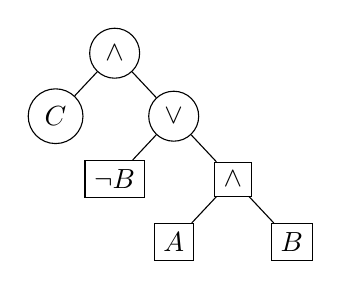
\begin{tikzpicture}[level distance=0.8cm] % C \land [\neg B \lor (A \land B)]
      \node[draw,circle] {$\land$}
      child {node[draw,circle] {$C$}}
      child {node[draw,circle] {$\lor$}
        child {node[draw,rectangle] {$\neg B$}}
        child {node[draw,rectangle] {$\land$}
          child {node[draw,rectangle] {$A$}}
          child {node[draw,rectangle] {$B$}}
        }
      };
    \end{tikzpicture}
    \caption{d-DNNF}
    \label{fig:ddnnf}
  \end{subfigure}
  \begin{subfigure}{0.32\textwidth}
    \centering
    \begin{tikzpicture}[level distance=0.8cm]
      \tikzset{
        mysplit/.style={
          draw,
          rectangle,
          rectangle split,
          rectangle split horizontal,
          rectangle split parts=2
        }
      }
      \node[draw,circle] {$1$}
      child {node[mysplit] (bullet) {
          \nodepart{one} $\neg A$
          \nodepart{two}
        }
        child {node[draw,circle] (3) {$3$} edge from parent[draw=none]
          child {node[mysplit] {
              \nodepart{one} $\neg B$
              \nodepart{two} $C$
            }
          }
          child {node[mysplit] {
              \nodepart{one} $B$
              \nodepart{two} $\bot$
            }
          }
        }
      }
      child {node[mysplit] {
          \nodepart{one} $A$
          \nodepart{two} $C$
        }};
      \draw[*-] let \p1 = (bullet.two), \p2 = (bullet.center) in ({\x1 + 2.5},{\y2 + 2}) -- (3);
    \end{tikzpicture}
    \caption{SDD}
    \label{fig:sdd}
  \end{subfigure}
  \begin{subfigure}{0.32\textwidth}
    \centering
    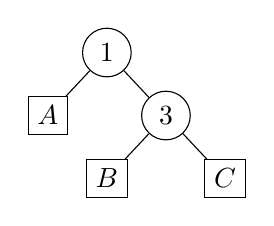
\begin{tikzpicture}[level distance=0.8cm]
      \node[draw,circle] {$1$}
      child {node[draw,rectangle] {$A$}}
      child {node[draw,circle] {$3$}
        child {node[draw,rectangle] {$B$}}
        child {node[draw,rectangle] {$C$}}
      };
    \end{tikzpicture}
    \caption{vtree}
    \label{fig:vtree}
  \end{subfigure}
  \caption{A d-DNNF and an SDD representation of $C \land (A \lor \neg B)$, together with the corresponding vtree. The numbers 1 and 3 come from the in-order traversal of the vtree and visually connect subtrees of both the SDD and the vtree.}
  \label{fig:kc}
\end{figure}

Note that the formulas in \cref{example:ddnnf1,example:ddnnf2} are equivalent, and the latter is also pictured in \cref{fig:ddnnf}.

Next, to define SDDs, we first need to define vtrees.

\begin{definition}[\citep{DBLP:conf/aaai/PipatsrisawatD08}]
  A \emph{vtree} for a set of variables $X$ is a full binary tree $T$ with a bijection between $X$ and the leaves of $T$.
\end{definition}

Let $\langle\cdot\rangle$ denote the function that maps an SDD to the propositional formula that it represents.

\begin{definition}[\citep{DBLP:conf/ijcai/Darwiche11}]
  Let $V$ be a vtree for a set of variables $X$. Then $S$ is an \emph{SDD} that respects $V$ if one of the following is true:
  \begin{itemize}
  \item $S = \bot$ ($\langle \bot \rangle \coloneqq \bot$);
  \item $S = \top$ ($\langle \top \rangle \coloneqq \top$);
  \item $S = x$, or $S = \neg x$, where $x \in X$ is the variable bijectively associated with the \emph{only} node of $V$ ($\langle x \rangle \coloneqq x$, and $\langle \neg x \rangle \coloneqq \neg x$);
  \item $S = \{\, (p_i, s_i) \mid i = 1, \dots, n \,\}$ for some $n \ge 1$, where \emph{primes} $\{\,p_i\,\}_{i=1}^n$ and \emph{subs} $\{\,s_i\,\}_{i=1}^n$ are SDDs such that:
    \begin{itemize}
    \item $V$ has more than one node,
    \item each $p_i$ respects the left subtree of $V$,
    \item each $s_i$ respects the right subtree fo $V$.
    \item the primes form a \emph{partition}, i.e.:
      \begin{itemize}
      \item $\langle p_i \rangle \not\equiv \bot$ for all $i = 1, \dots, n$ (i.e., the primes are \emph{consistent}),
      \item $\langle p_i \rangle \land \langle p_j \rangle \equiv \bot$ for all $i \ne j$ (i.e., the primes are \emph{mutually exclusive}),
      \item and $\bigvee_{i=1}^n \langle p_i \rangle \equiv \top$
      \end{itemize}
    \end{itemize}
    (then $\langle S \rangle \coloneqq \bigvee_{i=1}^n \langle p_i \rangle \land \langle s_i \rangle$).
  \end{itemize}
\end{definition}

\begin{example}
  Let $S = \{\, (A, C), (\neg A, \{\, (\neg B, C), (B, \bot) \,\}) \,\}$. Then $S$ (as pictured in \cref{fig:sdd}) is an SDD representation of $C \land (A \lor \neg B)$ that respects the vtree in \cref{fig:vtree}. Indeed,
  \begin{align*}
    \langle S \rangle &= (A \land C) \lor (\neg A \land [(\neg B \land C) \lor (B \land \bot)]) \\
    &\equiv (A \land C) \lor (\neg A \land \neg B \land C) \\
    &\equiv C \land (A \lor [\neg A \land \neg B]) \\
    &\equiv C \land ([A \lor \neg A] \land [A \lor \neg B]) \\
    &\equiv C \land (\top \land [A \lor \neg B]) \\
    &\equiv C \land (A \lor \neg B).
  \end{align*}
\end{example}

A BDD is similar to a decision tree that ends with either one or zero but generalised to a directed acyclic graph.

Both d-DNNF and SDD are normal forms for propositional formulae that satisfy certain properties.

\begin{figure}
  \centering
  \begin{subfigure}{0.18\textwidth}
    \centering
    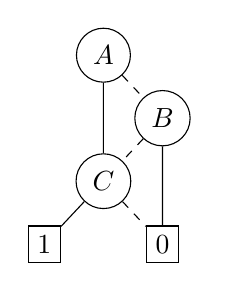
\begin{tikzpicture}[level distance=0.8cm]
      \node[draw,circle] (A) {$A$}
      child {edge from parent[draw=none]}
      child {node[draw,circle] (B) {$B$} edge from parent[dashed]
        child {node[draw,circle,solid] (C) {$C$} edge from parent[dashed]
          child {node[draw,rectangle,solid] {$1$} edge from parent[solid]}
          child {node[draw,rectangle,solid] (0) {$0$}}
        }
        child {edge from parent[draw=none]}
      };
      \draw (A) -- (C);
      \draw (B) -- (0);
    \end{tikzpicture}
    \caption{BDD}
    \label{fig:bdd}
  \end{subfigure}
  \begin{subfigure}{0.20\textwidth}
    \centering
    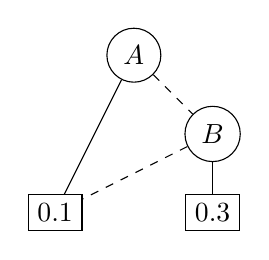
\begin{tikzpicture}
      \node[circle,draw] (x) at (0, 0) {$A$};
      \node[circle,draw] (y) at (1, -1) {$B$};
      \node[draw] (a) at (-1, -2) {0.1};
      \node[draw] (b) at (1, -2) {0.3};
      \draw[dashed] (x) -- (y);
      \draw (x) -- (a);
      \draw[dashed] (y) -- (a);
      \draw (y) -- (b);
    \end{tikzpicture}
    \caption{ADD}
    \label{fig:add}
  \end{subfigure} % TODO: could redraw the third diagram to be more like the others
\end{figure}

BDDs are a strict subset of SDDs that are a strict subset of d-DNNF \citep{DBLP:conf/ijcai/Darwiche11}.

Similarly to how BDDs represent Boolean functions, ADDs represent pseudo-Boolean functions, i.e., while (non-trivial) BDDs always have two sinks marked with one and zero, ADDs can have any number of sinks that contain, typically, real numbers \citep{DBLP:journals/fmsd/BaharFGHMPS97}.

ADDs have been extended to represent the additive and multiplicative structure in sink values more compactly \citep{DBLP:conf/ijcai/SannerM05} and to support first-order logic \citep{DBLP:journals/ai/SannerB09} and continuous variables \citep{DBLP:conf/uai/SannerDB11}.

ADDs have been used to represent the value functions of Markov decision processes \citep{DBLP:conf/uai/HoeySHB99} and probabilities in PGMs \citep{DBLP:conf/ijcai/ChaviraD07,DBLP:conf/uai/GogateD11}.

\begin{itemize}
\item maybe add a vtree for the SDD from the slides? I think the vtree is wrong...
\item have an example of an SDD in its set-of-sets-of...of literals and top/bot.
\item say: These formulas are often interpreted as trees or DAGs.
\item TODO: add info from the random slides, Chapter 5, and the full KR paper. But how much?
\item explain why the focus is on representations of propositional formulas and pseudo-Boolean functions
\item Boolean and Pseudo-Boolean Functions
\item NNF and how d-DNNF restricts that
\item A graphical representation of the ADD from ??. Sinks are represented as rectangles and other nodes as circles. The labels of nodes are written directly on them. An edge $e$ is dashed if $\epsilon(e) = 0$ and solid otherwise.
\item advertise \citep{DBLP:journals/jair/DarwicheM02} as a description of many normal forms and representations
\end{itemize}

\section{Applications}

of WMC?

copy info from my year 2 report

\begin{itemize}
\item Statistical Relational Learning
\item Neuro-Symbolic Artificial Intelligence
\item Natural Language Processing
\item Robotics
\end{itemize}
 % 11-45 pages (27 on average)
%% \include{cp}
%% \include{uai}
%% \include{sat}
%% \include{parameters}
%% \include{firstorder}
% >= 5 pages
\chapter{Conclusion}\label{chapter:conclusion}

In \cref{sec:contributions} we review the contributions of this thesis, and in
\cref{sec:future} we provide a perspective on how future work could develop,
either directly or indirectly based on the results of our work.

\section{Contributions}\label{sec:contributions}
% ================================= CONTRIBUTIONS (reiterating their importance) =================================
% how have I improved the state of the art?
% what do we understand better as a consequence of my work?
% recurring themes?
% claims?
% what broad areas of research are affected by my work? how might that effect propagate in the future?

% Recall that WMC is a fundamental computational task underlying many formalisms
% and applications.

The contributions of this thesis can be divided into two parts:
\begin{itemize}
  \item empirically-motivated contributions that make WMC more efficient
  \item and (conceptual, theoretical, or experimental) contributions that help
        us understand WMC (more fully or in a new way).
\end{itemize}

% ================================= EMPIRICAL STATE OF THE ART =================================

On the empirical front, most of our contributions focus on the efficiency and
tractability of the propositional and first-order variants of WMC\@. In
\cref{chapter:wmc1,chapter:wmc2}, we show how the efficiency of WMC can be
improved by generalising weights from their standard definition based on
literals to one capable of representing a richer subset of all possible
pseudo-Boolean functions. In \cref{chapter:wfomc}, we extend the capabilities of
\textsc{ForcLift} \citep{DBLP:conf/ijcai/BroeckTMDR11} so that it can solve more
instances in a lifted manner, e.g., instances with injective mappings. The
empirical contributions of \cref{chapter:randomlps,chapter:comparison} are about
introducing novel tools and methods for WMC\@. In \cref{chapter:randomlps}, we
developed a constraint model for (probabilistic) logic programs that can be used
to generate random programs or enumerate all small programs under some given
constraints. The constraints include various notions of size, the
structure/complexity of a clause, and the independence of random variables.
Finally, in \cref{chapter:comparison}, we present a way to generate
propositional formulas in CNF with varying primal treewidth. As treewidth is a
well-known parameter commonly used to describe parameterised complexity results
\citep{DBLP:series/txcs/DowneyF13}, the same model (or a variation thereof) can
be used in experimental studies of many other logic-based problems as well.

% ================================= UNDERSTANDING =================================

The experimental work in these last two chapters, i.e.,
\cref{chapter:randomlps,chapter:comparison}, also contains important
observations about WMC and probabilistic inference algorithms. First,
\cref{chapter:randomlps} demonstrates remarkable similarities among ProbLog
inference algorithms. This observation suggests that the bottleneck of ProbLog
inference (at least across our random instances) might be related to logic
programming more than WMC\@. Second, \cref{chapter:comparison} reveals, among
other things, that WMC algorithms based on algebraic decision diagrams (ADDs)
and dynamic programming scale worse with primal treewidth and work better with
instances that have fewer clauses (i.e., lower density) compared to other
algorithms. Understanding such differences among algorithms is important in the
development of new algorithms, algorithm portfolios, and hybrid approaches to
WMC\@. Back in \cref{chapter:wmc1}, we show how WMC can be seen as the problem
of computing the value of a measure on some element of a Boolean algebra. This
insight leads us to consider generalised weight functions that express, e.g.,
conditional probabilities more succinctly and can lead to improved probabilistic
inference speed for Bayesian networks. In \cref{chapter:wmc2}, we continue the
work on generalising WMC and formally define the generalisation as
pseudo-Boolean projection (PBP). Moreover, we show that previous work on WMC
encodings is not in vain, and the benefits can (in most cases) be transferred to
PBP\@. Lastly, \cref{chapter:wfomc} contains two important lessons. First,
`circuits' with cycles can be more expressive than their acyclic predecessors.
Second, first-order model counting (and first-order knowledge compilation in
particular) can discover the definitions of recursive functions (including
recurrence relations) that capture the model count of a given sentence.

In summary, we
\begin{itemize}
  \item introduced new foundations for WMC based on measures on Boolean
        algebras,
  \item generalised WMC to PBP,
  \item introduced new encoding schemes and encoding transformation algorithms,
  \item introduced \textsc{Crane}, i.e., a more powerful version of
        \textsc{ForcLift} that works with graphs rather than circuits,
  \item and provided algorithms for random instance generation.
\end{itemize}

%% \section{Discussion}

%% While WMC and its counterpart for first-order logic WFOMC both take
%% logic-based input and compute a sum of products, algorithmically they are
%% quite different. The first difference is in the size of input: most WFOMC
%% benchmarks have at most three variables whereas most WMC instances have
%% thousands of variables. This difference motivates the definition of
%% liftability in lieu of tractability. Let us take DPMC
%% \citep{DBLP:conf/cp/DudekPV20} and \textsc{ForcLift} as representative
%% examples of algorithms for each problem. The way in which an algorithm solves
%% an instance can be explained as a sequence of operations: on ADDs in the
%% former case and on (a variation of) formulas in the latter. However, due to
%% the difference in input size, WMC algorithms are expected to perform a much
%% larger number of such operations. Hence, the efficiency of each individual
%% operation is more important in the case of WMC. Here, optimising not just the
%% asymptotic complexity of each operation but also the data structures in use
%% can yield significant performance gains. Finally, there is an important
%% difference regarding complexity. As is the case with all complete exact
%% solutions to \NP-hard problems, WMC algorithms have an exponential worst-case
%% complexity. A typical algorithm attempts to do much better on most realistic
%% instances, but provides no guarantees. In contrast, one can often express the
%% running time of a WFOMC algorithm on an instance $\mathscr{I}$ as
%% $\Theta(p(n_1, \dots, n_k))$, where $p$ is a polynomial, and
%% $\{\,n_i\,\}_{i=1}^k$ are the sizes of the domains in $\mathscr{I}$.

%% Algorithmically, W(FO)MC is interesting because of its connections to classic
%% decision problems such as SAT, counting problems like \mc{}, and other
%% function problems such as polynomial evaluation. The algorithms benefit from
%% many disparate techniques such as dynamic programming
%% \citep{DBLP:conf/aaai/DudekPV20,DBLP:conf/cp/DudekPV20}, knowledge
%% compilation \citep{DBLP:conf/ecai/Darwiche04,DBLP:conf/ijcai/BroeckTMDR11},
%% search \citep{DBLP:conf/sat/SangBBKP04,DBLP:conf/ijcai/BroeckTMDR11}, tree
%% decompositions \citep{DBLP:conf/cp/DudekPV20,DBLP:conf/cp/KorhonenJ21}, and
%% close collaboration with SAT algorithms
%% \citep{DBLP:conf/ecai/Darwiche04,DBLP:conf/ijcai/LagniezM17,DBLP:conf/sat/SangBBKP04}.

%% We hope that the contributions in this thesis will...

%% \paragraph*{Impact: What broad areas of research are affected by my work?}
%% \begin{itemize}
%% \item theory and algorithms: counting algorithms, arithmetic complexity
%% \item AI: PGMs, statistical relational learning
%% \end{itemize}

\section{Future Directions}\label{sec:future}
%% approximate DPMC: cite the APRICODD paper
%% \citep{DBLP:conf/nips/St-AubinHB00}. Also, if two sinks have very similar
%% values, an approximation could merge them

In this section, we present a broad overview of how our contributions and the
questions raised by this work could be taken forward and influence key areas of
research in computer science, artificial intelligence (AI), and mathematics.

\subsection{Algorithms and Applications}

% You could mention the use of portfolio approaches to make SAT extremely fast
% \citep{DBLP:journals/jair/XuHHL08} (other domains
% \citep{DBLP:conf/lion/KotthoffMS16}), and whether something similar could be
% tried out with your work.

In this thesis, we contributed to the development and applicability of three WMC
algorithms: \textsc{ADDMC} \citep{DBLP:conf/aaai/DudekPV20}, \textsc{DPMC}
\citep{DBLP:conf/cp/DudekPV20}, and \textsc{ForcLift}
\citep{DBLP:conf/ijcai/BroeckTMDR11}. The first two are propositional WMC
algorithms based on ADDs, whereas \textsc{ForcLift} is a WMC algorithm for
first-order logic based on knowledge compilation. While in this work we focused
exclusively on exact algorithms, all of them could be adapted to approximate
instead. An approximation technique called \emph{lifted relax, compensate and
  then recover} is already part of \textsc{ForcLift}
\citep{DBLP:conf/uai/BroeckCD12}, so it would only need to be adapted to the
generalised setting of \textsc{Crane}. Likewise, approximate computations using
ADDs have already been studied \citep{DBLP:conf/nips/St-AubinHB00}, so, e.g.,
\textsc{DPMC} could be extended to approximate as well.

Most weighted first-order model counting (WFOMC) algorithms try to solve each
instance in a lifted manner (i.e., run in polynomial time with respect to the
sizes of the domains involved) and fail if unsuccessful. \textsc{ForcLift} is an
exception as it supports using a (propositional) WMC algorithm for parts of the
problem that cannot be solved by other compilation rules. Can this transition to
WMC be implemented more efficiently, i.e., without fully grounding the instance?
Is the WFOMC algorithm better off constructing its own exponential-time solution
instead of relying on a WMC algorithm (and is that even possible)? The only way
WFOMC can become the standard approach to probabilistic inference in statistical
relational models is by being able to gracefully handle all instances, even if
it means abandoning efficiency guarantees.

Finally, ample opportunities remain to improve WMC encodings that already exist
as well as connect WMC to new problem domains. In particular, we showed how PBP
encodings of Bayesian networks are much smaller than the equivalent WMC
encodings and can be handled more efficiently by a WMC algorithm. Designing PBP
encodings for other applications of WMC and new problem domains could be
similarly beneficial. Moreover, back in \cref{chapter:introduction}, we compared
WMC to a range of other computational problems that ask to compute a sum of
products. Establishing efficient reductions among these problems could yield new
fixed-parameter tractable algorithms and/or improvements to the empirical state
of the art. Similarly, adapting a WMC algorithm to a semiring other than
$(\mathbb{R}_{\ge 0}, +, \cdot)$ could yield improvements to some of the related
problems outlined by \citet{DBLP:journals/japll/KimmigBR17}.

\subsection{Computational Complexity}

Note that the execution of both WMC and WFOMC algorithms can be divided into two
parts:
\begin{itemize}
  \item looking for a \emph{solution} (i.e., an arithmetic circuit/expression
        that computes the required sum of products) and
  \item performing the numerical computations that produce the final answer.
\end{itemize}
(The two are typically much more intertwined in the case of propositional WMC.)
With this dichotomy in mind, one could ask: are the algorithms finding optimal
solutions? How much of the total running time depends on the complexity of the
solution, and how much on the algorithmic methods for finding one? Answers to
these questions would highlight the weaknesses of state-of-the-art algorithms
and direct the efforts of future research towards addressing these weaknesses.

On a more theoretical level, single-domain (W)FOMC problems compute sequences,
many of which are well-known to mathematicians. Since there is significant
interest in computing such sequences efficiently, the existence of many such
sequences with no efficient formulas suggests that a tractable solution might
not exist. However, we have no proof of that, i.e., no arithmetic circuit lower
bounds for sequences that have been known for decades and are easy to describe
in natural language and logic. So far, the most notable hardness result
states that there exists a sentence in first-order logic with three variables
for which FOMC is $\#\P_1$-complete \citep{DBLP:conf/pods/BeameBGS15}. Having
similar hardness results for sentences that are both simple and practical would
be a significant advancement in the field.

\subsection{Random Instances}

In this thesis, we introduce two ways to generate random instances: one for
(probabilistic) logic programs and one for propositional formulas in CNF that
are then turned into WMC instances. As we provide the very first attempts at
testing WMC algorithms on random data, many opportunities for improvements and
future work remain.

To begin with, applications of WMC could inspire future work on random instance
generation in two ways. First, one could generate random instances of some
application of WMC and convert them to WMC instances or probabilistic logic
programs. Second, one could analyse the properties of real-world data and
develop random models that exhibit similar characteristics as has been done
quite extensively in the SAT community
\citep{DBLP:conf/ijcai/AnsoteguiBL09,DBLP:conf/tacas/BlasiusFS19,DBLP:journals/ai/Giraldez-CruL16,DBLP:conf/ijcai/Giraldez-CruL17}.

Moreover, an interesting opportunity to connect our work on random logic
programs in \cref{chapter:randomlps} and on (W)FOMC in \cref{chapter:wfomc} is
by adapting the constraint model to generate (W)FOMC instances instead of logic
programs. This way one could systematically search for interesting instances
that, e.g.,
\begin{itemize}
  \item reveal differences in the runtime complexity of various algorithms or
  \item demonstrate a gap between the performance of state-of-the-art WFOMC
        algorithms and formulas constructed by hand.
\end{itemize}

There is also ample opportunity for theoretical contributions. For instance, one
explanation for the surprising experimental results of \cref{chapter:randomlps}
is that all of the generated instances yielded easy WMC problems, and the
computational bottleneck was in the handling of the logic program before WMC\@.
We can state this idea as a (somewhat informal) conjecture.

\begin{conjecture}
  With high probability, the WMC instance that results from a random
  probabilistic logic program generated by the constraint model in
  \cref{chapter:randomlps} is tractable for some WMC algorithm.
\end{conjecture}

%% random CNFs with bounds on primal treewidth (what makes it tricky in my case
%% is that one random decision influences/conditions all subsequent decisions,
%% unlike in the case of Erd\H{o}s-R\'enyi random graphs)

\subsection{Artificial Intelligence and Combinatorics}

A swiftly emerging area of research---neural-symbolic AI---attempts to combine
deep neural networks (the approach to machine learning responsible for many
recent achievements in the field) with logical reasoning
\citep{DBLP:conf/ijcai/RaedtDMM20,garnelo2019reconciling,DBLP:series/faia/342}.
As a result, explicit background knowledge can be seamlessly integrated with
large amounts of low-level data that deep neural networks are so proficient at
handling. Similarly, our hope for the broader field of AI is that the field
shifts some of its focus from numbers and probabilities to structural concepts
such as functions and relations. Once a solution to, e.g., a WFOMC problem is
formulated as a function $f$ rather than the evaluation of $f$ on some
particular input values, richer ways of reasoning become available. For example,
instead of asking whether a probability of some event is above/below some
threshold in a particular situation, one could ask for conditions on the input
values that are necessary for the probability to be sufficiently high/low. Such
reasoning capabilities have clear benefits to the robustness of artificial
agents and explainability---another rapidly emerging area of research
\citep{DBLP:journals/corr/abs-1909-03012,DBLP:journals/fdata/BelleP21,DBLP:journals/corr/abs-2202-10335}.

For the benefit of both AI and combinatorics, we would like to reiterate and
expand on the notion of an automatic enumerative combinatorialist by
\citet{DBLP:conf/ilp/BarvinekB0ZK21}. Perhaps (W)FOMC can mature into an
easy-to-use tool that can compute any function expressible in first-order logic,
in many cases providing a simple solution via a combination of recursive
functions. Similarly to how a constraint programmer describes the constraints
and asks the solver for a solution, a combinatorialist could describe what needs
to be counted in a logic-based format and receive recursive or asymptotic
solutions, generating functions, etc.

% Instead there has been some recent work on making connections between tractable
% circuits and explainability, and perhaps you can articulate something based on
% that.
%   \begin{itemize}
%     \item use of tractable circuits in explainability and verification of neural
%           networks \citep{DBLP:conf/pods/Darwiche20}
%     \item some of the tractable circuits are essentially WMC encodings
%           \citep{DBLP:conf/nips/ShenCD16}
%   \end{itemize}

%% Many open questions remain about the capabilities of logic-based methods for counting and performing sum-of-products computations, particularly in the context of first-order logic. The answer to a WFOMC instance depends on three things: the formula, the weights, and the domain sizes. By fixing the first two, the instance becomes a logical representation of a function $\mathbb{N}_0^n \to \mathbb{R}_{\ge 0}$, where $n$ is the number of domains. In particular, an unweighed formula $\phi$ that depends on only one domain $\Delta$ represents an integer sequence that we get by computing the model count of $\phi$ across all possible cardinalities of $\Delta$. This observation raises important open questions with the potential to improve WFOMC algorithms, contribute to other counting problems and find new efficiently-computable formulas to sequences of interest.

%% First, how complete is first-order logic in its ability to describe such functions? Can we identify conditions (e.g., monotonicity) that must be satisfied by a function for it to be representable as an instance of WFOMC? Can we find examples of simple sequences that are provably unrepresentable? Would a different kind of logic (e.g., second-order or modal) be more complete in this way? Answering these questions could help identify new areas of application of WFOMC and ensure that instances that are solvable in theory can be solved in practice as well.

%% Second, instead of finding (a more complex type of) arithmetic circuits that compute functions from their logical descriptions, is it possible to go in the other direction? That is, can we identify logical gadgets for all algebraic operations that could then be combined to form a WFOMC representation of a given function? This way, WFOMC could be used to automatically reformulate, e.g., functions that use an exponential amount of recursive calls to more tractable expressions.

%% Third, if a WFOMC algorithm identifies a recursive function (or a recurrence relation) as part of the solution, can we use one of the many recurrence-relation-solving techniques to replace recursive computations with a closed-form solution? More generally, there is ample opportunity to expand the set of algorithmic techniques and algebraic constructions used in WFOMC to one that is more complete (i.e., able to construct tractable solutions) and efficient. For instance, the use of negation is currently limited to Skolemization (i.e., removal of existential quantification), but one can construct instances whose most efficient solutions feature powers of negative one despite the formula having no existential quantification. Similarly to \cref{chapter:wfomc}, this could further extend the set of instances that can be handled in a lifted (i.e., tractable with respect to domain sizes) manner and improve the complexity of solutions that are already tractable.
 % 5-28 pages (mean: 8, median: 5)

%% \appendix
%% \include{appendix1}

%% Choose your favourite bibliography style here.
\bibliographystyle{apalike}

%% If you want the bibliography single-spaced (which is allowed), uncomment
%% the next line.
% \singlespace

\bibliography{thesis}

\end{document}
